%--------------------------------------------------------------------------------------
% Dokumentum formátuma [Document format]
%--------------------------------------------------------------------------------------

%TODO Válaszd ki, hogy egyoldalas vagy kétoldalas legyen! [Choose format]
\documentclass[12pt,a4paper,oneside]{report}             % Egyoldalas [Single-side]
%\documentclass[12pt,a4paper,twoside,openright]{report}  % Kétoldalas [Duplex]


%--------------------------------------------------------------------------------------
% Csomagok inicializálása [Initializing packages]
%--------------------------------------------------------------------------------------
\usepackage{ifthen} % Used in macros

\usepackage[english,magyar]{babel} % Language support
\usepackage{geometry}
\usepackage{amsfonts,amsmath,amssymb} % Mathematical symbols
\usepackage{microtype} % Imrovements to typesetting
\usepackage{setspace} % For setting line spacing
\usepackage{cmap} % Enables more advenced text copying from the PDF document
\usepackage{sectsty} % Section heading styling

\usepackage[unicode]{hyperref} % For hyperlinks in the generated document
\usepackage{booktabs} % For publication quality tables for LaTeX
\usepackage{graphicx} % For figure sizing
\usepackage[hang]{caption}
\usepackage{xcolor} % For code coloring in listings
\usepackage{listings} % For source code snippets
\usepackage[amsmath,thmmarks]{ntheorem} % Theorem-like environments

\usepackage[numbers]{natbib} % Bibliography

%\usepackage{fancyhdr} % For easy to use headers and footers

% thanks to http://tex.stackexchange.com/a/47579/71109
\usepackage{ifxetex}
\usepackage{ifluatex}
\newif\ifxetexorluatex % a new conditional starts as false
\ifnum 0\ifxetex 1\fi\ifluatex 1\fi>0
  \xetexorluatextrue
\fi

\ifxetexorluatex
  \usepackage{fontspec}
  % Palatino clone font (Tex Gyre Pagella) for text and math
  \usepackage{newpxmath}
  \setmainfont[Ligatures=TeX]{TeX Gyre Pagella}
\else
  \usepackage[T1]{fontenc}
  \usepackage[utf8]{inputenc}
  %\usepackage[lighttt]{lmodern} % Advanced version of the Computer Modern font
  % Palatino clone font (Tex Gyre Pagella) for text and math
  \usepackage{tgpagella, newpxmath}
\fi

\usepackage{titlesec} % removeme
\usepackage{subfig}  % removeme
\usepackage{svg}


%--------------------------------------------------------------------------------------
% Dokumentum nyelve [Language]
%--------------------------------------------------------------------------------------

%TODO Válaszd ki a nyelvet! [Select language]
\input{include/language-setup-hu} % Beállítások magyar nyelvű dolgozathoz
%\input{include/language-setup-en}    % Settings for English document

% Megjegyzés:
%         Ez a beállítás az automatikusan létrehozott címek, hivatkozások
%         nyelvét adja meg, valamint a nyelvre jellemző behúzási távolságot
%         használja a bekezdések elején.
%
% Note:
%         This setting controls the language of generated titles and citations,
%         moreover the paragraph indentation.


%--------------------------------------------------------------------------------------
% Preambulum (LaTeX beállítások, makrók) [Preamble (LaTeX settings)]
%--------------------------------------------------------------------------------------
%--------------------------------------------------------------------------------------
% Page layout setup
%--------------------------------------------------------------------------------------
% we need to redefine the pagestyle plain
% another possibility is to use the body of this command without \fancypagestyle
% and use \pagestyle{fancy} but in that case the special pages
% (like the ToC, the References, and the Chapter pages)remain in plane style

\pagestyle{plain}
\geometry{inner=30mm, outer=20mm, top=20mm, bottom=30mm}


%--------------------------------------------------------------------------------------
% Text and paragraph styling
%--------------------------------------------------------------------------------------

\sectionfont{\Large\upshape\bfseries}  % Section title font
\subsectionfont{\Large\itshape\mdseries}
\subsubsectionfont{\large\itshape\mdseries}
\setcounter{secnumdepth}{3}             % Section numbering depth

\sloppy                                 % Prevent text from spilling over the margin
\widowpenalty=10000 \clubpenalty=10000  % Prevent widow and oprhan rows
\def\hyph{-\penalty0\hskip0pt\relax}    % Enable hyphenation

\onehalfspacing                         % 1.5x Line spacing

% Text setup for Hungarian text
\newcommand{\selecthungarian}{
	\selectlanguage{magyar}
	\setlength{\parindent}{2em}			% Paragraph indentation
	\setlength{\parskip}{5pt}			% Paragraph spacing
	\frenchspacing
}

% Text setup for English text
\newcommand{\selectenglish}{
	\selectlanguage{english}
	\setlength{\parindent}{0em}
	\setlength{\parskip}{8pt}
	\nonfrenchspacing
}

%--------------------------------------------------------------------------------------
% Setup hyperref package
%--------------------------------------------------------------------------------------
\hypersetup{
	% bookmarks=true,            % show bookmarks bar?
	unicode=true,                % non-Latin characters in Acrobat's bookmarks
	pdfnewwindow=true,           % links in new window
	colorlinks=true,             % false: boxed links; true: colored links
	linkcolor=black,             % color of internal links
	citecolor=black,             % color of links to bibliography
	filecolor=black,             % color of file links
	urlcolor=black               % color of external links
}

%--------------------------------------------------------------------------------------
% Apply variables
%--------------------------------------------------------------------------------------
% This command is called in the main tex file and uses variables set there.
\newcommand{\applyvariables}{
	\author{\authorName}
	\title{\thesisTitle}

	\hypersetup{
		pdftitle={\thesisTitle},     % title
		pdfauthor={\authorName},     % author
		pdfsubject={\gpkmunkatipus}, % subject of the document
		pdfkeywords={\keywords},     % list of keywords (separate then by comma)
		pdfproducer={\authorName},   % producer of the document (organization)
		pdfcreator={LaTeX}           % creator of the document (application)
	}
}

%--------------------------------------------------------------------------------------
% Set up listings
%--------------------------------------------------------------------------------------
\definecolor{lightgray}{rgb}{0.95,0.95,0.95}
\lstset{
basicstyle=\scriptsize\ttfamily, % print whole listing small
keywordstyle=\color{black}\bfseries, % bold black keywords
identifierstyle=, % nothing happens
% default behavior: comments in italic, to change use
% commentstyle=\color{green}, % for e.g. green comments
stringstyle=\scriptsize,
showstringspaces=false, % no special string spaces
aboveskip=3pt,
belowskip=3pt,
backgroundcolor=\color{lightgray},
columns=flexible,
keepspaces=true,
escapeinside={(*@}{@*)},
captionpos=b,
breaklines=true,
frame=single,
float=!ht,
tabsize=2,
literate=*
	{á}{{\'a}}1	{é}{{\'e}}1	{í}{{\'i}}1	{ó}{{\'o}}1	{ö}{{\"o}}1	{ő}{{\H{o}}}1	{ú}{{\'u}}1	{ü}{{\"u}}1	{ű}{{\H{u}}}1
{Á}{{\'A}}1	{É}{{\'E}}1	{Í}{{\'I}}1	{Ó}{{\'O}}1	{Ö}{{\"O}}1	{Ő}{{\H{O}}}1	{Ú}{{\'U}}1	{Ü}{{\"U}}1	{Ű}{{\H{U}}}1
}


%--------------------------------------------------------------------------------------
% Set up theorem-like environments
%--------------------------------------------------------------------------------------
% Using ntheorem package -- see http://www.math.washington.edu/tex-archive/macros/latex/contrib/ntheorem/ntheorem.pdf

\theoremstyle{plain}
\theoremseparator{.}
\newtheorem{example}{\pelda}

\theoremseparator{.}
%\theoremprework{\bigskip\hrule\medskip}
%\theorempostwork{\hrule\bigskip}
\theorembodyfont{\upshape}
\theoremsymbol{{\large \ensuremath{\centerdot}}}
\newtheorem{definition}{\definicio}

\theoremseparator{.}
%\theoremprework{\bigskip\hrule\medskip}
%\theorempostwork{\hrule\bigskip}
\newtheorem{theorem}{\tetel}


%--------------------------------------------------------------------------------------
% Some new commands and declarations
%--------------------------------------------------------------------------------------
\newcommand{\code}[1]{{\upshape\ttfamily\scriptsize\indent #1}}
\newcommand{\doi}[1]{DOI: \href{http://dx.doi.org/\detokenize{#1}}{\raggedright{\texttt{\detokenize{#1}}}}} % A hivatkozások közt így könnyebb DOI-t megadni.

\DeclareMathOperator*{\argmax}{arg\,max}
%\DeclareMathOperator*[1]{\floor}{arg\,max}
\DeclareMathOperator{\sign}{sgn}
\DeclareMathOperator{\rot}{rot}


%--------------------------------------------------------------------------------------
% Setup captions
%--------------------------------------------------------------------------------------
\captionsetup[figure]{
	width=.75\textwidth,
	aboveskip=10pt}

\renewcommand{\captionlabelfont}{\it}
\renewcommand{\captionfont}{\footnotesize\it}

%--------------------------------------------------------------------------------------
% Hyphenation exceptions
%--------------------------------------------------------------------------------------
\hyphenation{Shakes-peare Mar-seilles ár-víz-tű-rő tü-kör-fú-ró-gép}


%--------------------------------------------------------------------------------------
% Command to exclude tables and images in the annex from the List of Figures/Tables
%--------------------------------------------------------------------------------------
\newcommand{\excludeFromLocAndLot}{
	% Redefine \addcontentsline to be silent when printing loc or toc entries
	\let\svaddcontentsline\addcontentsline
	\renewcommand\addcontentsline[3]{
		\ifthenelse{\equal{##1}{lof}}{}{
			\ifthenelse{\equal{##1}{lot}}{}{
				\svaddcontentsline{##1}{##2}{##3}
			}
		}
	}
}


%--------------------------------------------------------------------------------------
% Munkatípus [Thesis type]
%--------------------------------------------------------------------------------------

%TODO Válaszd ki a munkatípust [Select thesis type]
% \selectbsc    % Szakdolgozat [Bachelor's]
\selectmsc   % Diplomaterv [Master's]


%--------------------------------------------------------------------------------------
% Változók beállítása [Setting variables]
%--------------------------------------------------------------------------------------

%TODO Állítsd be az alábbi változókat [Set these variables]

% Szerző [Author]
\def\authorFamilyName{László}
\def\authorGivenName{Máté}
\def\neptun{K9QU7H}

% Konzulens 1 [Consulent 1]
\def\consulentATitle{}
\def\consulentAFamilyName{Dudás}
\def\consulentAGivenName{ávid}
\def\consulentARank{óraadó}

% Konzulens 2 [Consulent 2], ha nincs hagyd üresen
\def\consulentBTitle{}
\def\consulentBFamilyName{}
\def\consulentBGivenName{}
\def\consulentBRank{}

% Konzulens 3 [Consulent 3], ha nincs hagyd üresen
\def\consulentCTitle{}
\def\consulentCFamilyName{}
\def\consulentCGivenName{}
\def\consulentCRank{}

% Témavezető
\def\supervisorTitle{dr.~}
\def\supervisorFamilyName{Budai}
\def\supervisorGivenName{Csaba}
\def\supervisorRank{tanszékvezető-helyettes, adjunktus}

% Dolgozat címe [Thesis title]
\def\thesisTitle{MPPI kontrollerhangolási módszer fejlesztése ROS2 robot platformon}

% Kulcsszavak (a PDF-be) [Keywords (to PDF)]
\def\keywords{mechatronika, szabályozástechnika, robotika, ROS2, NAV2}

% Tanszék [Department]
%TODO Válassz az alábbiak közül
% \bmeatt    \bmeara  \bmeenergia  \bmeepget  \bmegtharom
% \bmemanuf  \bmehds  \bmemogi     \bmemm     \bmept
\def\department{\bmemogi}

%TODO Cseréld le a figures/tanszek_logo.pdf képet a tanszéked logójára!
%     [Replace figures/tanszek_logo.pdf with the logo of your department]

% Elzártan kezelendő dolgozat [Restricted access]
%TODO Töltsd ki a korlátozás lejártának dátumát!
%     [Fill in the end date of the restriction]
\def\endOfRestrictedAccess{... év ... hónap ... nap}


% Változók beállítása a PDF fájlhoz [Apply variables for the PDF file]
\applyvariables


%--------------------------------------------------------------------------------------
% Dokumentum törzse [Document body]
%--------------------------------------------------------------------------------------

\begin{document}

\pagenumbering{gobble}
\selectthesislanguage

% Címoldal [Titlepage]
\include{include/titlepage-thesis}  % Szakdolgozat/Diplomaterv címlap [Thesis]


% Copytightoldal [Copyright page]
%TODO Válaszd ki a megfelelőt! [Choose one]
\include{include/copyrightpage}               % Nyílt kezelésű [Open access]
%\include{include/copyrightpage-restricted}   % Elzárt kezelésű [Restricted access]


% Feladatkiírás [Project page]
%TODO A nyomtatott verzóban ne szerepeljen! [Remove before printing]
% \include{chapters/project}


% Nyilatkozatok [Declarations]
\include{include/declaration}

\selectthesislanguage
% Tartalomjegyzék [Table of Contents]
\setcounter{tocdepth}{3}  % Tartalomjegyzék mélysége [ToC depth]
\tableofcontents\vfill


% Ábrák és táblázatok jegyzéke [List of Figures, Tables]
%TODO Kommenteld ki, ha használni szeretnéd. [Uncomment to use]
%\listoffigures\addcontentsline{toc}{chapter}{\listfigurename}   % Ábrák jegyzéke - opcionális
%\listoftables\addcontentsline{toc}{chapter}{\listtablename}     % Táblázatok jegyzéke - opcionális


% Előszó [Preface]
%----------------------------------------------------------------------------
\chapter*{\eloszo}\addcontentsline{toc}{chapter}{\eloszo}
%----------------------------------------------------------------------------

Az előszó legtöbbször személyes hangú, eligazító jellegű írás, amely a mű megírásának okairól, születésének körülményeiről szól. Az előszó nem szerves része a főszövegnek, hanem annak kiegészítése.
Ugyancsak az előszóban fejtheti ki a szerző a mű megértéséhez szükséges szempontokat, a követett módszereket, utalhat a fontosabb előzményekre és szakirodalomra.
Az előszó ne legyen terjedelmes.


Jelen dokumentum egy diplomaterv-sablon, amely formai keretet ad a BME Gépészmérnöki Karán végző hallgatók által elkészítendő szakdolgozatnak és diplomatervnek. A sablon használata opcionális. Ez a sablon \LaTeX~alapú, a \emph{TeXLive} \TeX-implementációval és a PDF-\LaTeX~fordítóval működőképes.
A sablon forrása a Mechatronika Szakosztály GitHub tárhelyén\footnotemark{} elérhető. Amennyiben hibát találtál, vagy észrevételed, javaslatod lenne, kérlek ott jelezd.

\footnotetext{\url{https://github.com/MechatronikaSzakosztaly/bme-gpk-thesis-latex}}

\begin{center}
    $\thicksim \; \thicksim \; \thicksim$
\end{center}



\subsubsection*{Köszönetnyilvánítás}
\emph{A köszönetnyilvánítás ide írható.} Ez a sablon a Villamosmérnöki és Informatikai Kar Méréstechnika és Információs Rendszerek Tanszék szakdolgozat és diplomaterv sablonja alapján készült. Köszönöm készítőinek és karbantartóinak a munkájukat.


\vspace{0.5cm}

\begin{flushleft}
    {Budapest, \today}
\end{flushleft}

\begin{flushright}
    \emph{\authorName}
\end{flushright}

\vfill



% Jelölések jegyzéke [Table of Symbols]
\include{chapters/symbols}


% Főszöveg [The main part of the thesis]
\cleardoublepage
\pagenumbering{arabic}
%TODO Importáld a saját fejezeteidet [Import your own content]
% \include{chapters/introduction}      % Bevezetés
% \include{chapters/latex-tools}       % 2. fejezet
% \include{chapters/thesis-format}     % 3. fejezet
% %----------------------------------------------------------------------------
\chapter{A \LaTeX-sablon használata}
%----------------------------------------------------------------------------

Ebben a fejezetben röviden, implicit módon bemutatjuk a sablon használatának módját, ami azt jelenti, hogy sablon használata ennek a dokumentumnak a forráskódját tanulmányozva válik teljesen világossá. Amennyiben a szoftver-keretrendszer telepítve van, a sablon alkalmazása és a dolgozat szerkesztése \LaTeX-ben a sablon segítségével tapasztalataink szerint jóval hatékonyabb, mint egy WYSWYG (\emph{What You See is What You Get}) típusú szövegszerkesztő esetén (pl. Microsoft Word, OpenOffice).

%----------------------------------------------------------------------------
\section{Címkék és hivatkozások}
%----------------------------------------------------------------------------
A \LaTeX~dokumentumban címkéket (\verb+\label+) rendelhetünk ábrákhoz, táblázatokhoz, fejezetekhez, listákhoz, képletekhez stb. Ezekre a dokumentum bármely részében hivatkozhatunk, a hivatkozások automatikusan feloldásra kerülnek.

A sablonban makrókat definiáltunk a hivatkozások megkönnyítéséhez. Ennek megfelelően minden ábra (\emph{figure}) címkéje \verb+fig:+ kulcsszóval kezdődik, míg minden táblázat (\emph{table}), képlet (\emph{equation}), fejezet (\emph{section}) és lista (\emph{listing}) rendre a \verb+tab:+, \verb+eq:+, \verb+sec:+ és \verb+lst:+ kulcsszóval kezdődik, és a kulcsszavak után tetszőlegesen választott címke használható. Ha ezt a konvenciót betartjuk, akkor az előbbi objektumok számára rendre a \verb+\figref+, \verb+\tabref+, \verb+\eqref+, \verb+\sectref+ és \verb+\listref+ makrókkal hivatkozhatunk. A makrók paramétere a címke, amelyre hivatkozunk (a kulcsszó nélkül). Az összes említett hivatkozástípus, beleértve az \verb+\url+ kulcsszóval bevezetett web-hivatkozásokat is a  \verb+hyperref+\footnote{Segítségével a dokumentumban megjelenő hivatkozások nem csak dinamikussá válnak, de színezhetők is, bővebbet erről a csomag dokumentációjában találunk. Ez egyúttal egy példa lábjegyzet írására.} csomagnak köszönhetően aktívak a legtöbb PDF-nézegetőben, rájuk kattintva a dokumentum megfelelő oldalára ugrik a PDF-néző vagy a megfelelő linket megnyitja az alapértelmezett böngészővel. A \verb+hyperref+ csomag a kimeneti PDF-dokumentumba könyvjelzőket is készít a tartalomjegyzékből. Ez egy szintén aktív tartalomjegyzék, amelynek elemeire kattintva a nézegető behozza a kiválasztott fejezetet.

%----------------------------------------------------------------------------
\section{Ábrák és táblázatok}
%----------------------------------------------------------------------------
Használjunk vektorgrafikus ábrákat, ha van rá módunk. PDFLaTeX használata esetén PDF formátumú ábrákat lehet beilleszteni könnyen, az EPS (PostScript) vektorgrafikus képformátum beillesztését a PDFLaTeX közvetlenül nem támogatja (de lehet konvertálni, lásd később). Ha vektorgrafikus formában nem áll rendelkezésünkre az ábra, akkor a  veszteségmentes PNG, valamint a veszteséges JPEG formátumban érdemes elmenteni.  Figyeljünk arra, hogy ilyenkor a képek felbontása elég nagy legyen ahhoz, hogy nyomtatásban is megfelelő minőséget nyújtson (legalább 300 dpi javasolt). A dokumentumban felhasznált képfájlokat a dokumentum forrása mellett érdemes tartani, archiválni, mivel ezek hiányában a dokumentum nem fordul újra. Ha lehet, a vektorgrafikus képeket vektorgrafikus formátumban is érdemes elmenteni az újrafelhasználhatóság (az átszerkeszthetőség) érdekében.

Kapcsolási rajzok legtöbbször kimásolhatók egy vektorgrafikus programba (pl. CorelDraw) és onnan nagyobb felbontással raszterizálva kimenthatők PNG formátumban. Ugyanakkor kiváló ábrák készíthetők Microsoft Visio vagy hasonló program használatával is: Visio-ból az ábrák közvetlenül PDF-be is menthetők.

Lehetőségeink Matlab ábrák esetén:
\begin{itemize}
	\item Képernyőlopás (\emph{screenshot}) is elfogadható minőségű lehet a dokumentumban, de általában jobb felbontást is el lehet érni más módszerrel.
	\item A Matlab ábrát a \verb+File/Save As+ opcióval lementhetjük PNG formátumban (ugyanaz itt is érvényes, mint korábban, ezért nem javasoljuk).
	\item A Matlab ábrát az \verb+Edit/Copy figure+ opcióval kimásolhatjuk egy vektorgrafikus programba is és onnan nagyobb felbontással raszterizálva kimenthatjük PNG formátumban (nem javasolt).
	\item Javasolt megoldás: az ábrát a \verb+File/Save As+ opcióval EPS \emph{vektorgrafikus} formátumban elmentjük, PDF-be konvertálva beillesztjük a dolgozatba.
\end{itemize}
Az EPS kép az \verb+epstopdf+ programmal\footnote{a korábban említett \LaTeX-disztribúciókban megtalálható} konvertálható PDF formátumba. Célszerű egy batch-fájlt készíteni az összes EPS ábra lefordítására az alábbi módon (ez Windows alatt működik).
\begin{lstlisting}[language=]
@echo off
for %%j in (*.eps) do (
  echo converting file "%%j"
  epstopdf "%%j"
)
echo done .
\end{lstlisting}

Egy ilyen parancsfájlt (\verb+convert.cmd+) elhelyeztük a sablon \verb+figures\eps+ könyvtárába, így a felhasználónak csak annyi a dolga, hogy a \verb+figures\eps+ könyvtárba kimenti az EPS formátumú vektorgrafikus képet, majd lefuttatja a \verb+convert.cmd+ parancsfájlt, ami PDF-be konvertálja az EPS fájlt.

Ezek után a PDF-ábrát ugyanúgy lehet a dokumentumba beilleszteni, mint a PNG-t vagy a JPEG-et. A megoldás előnye, hogy a lefordított dokumentumban is vektorgrafikusan tárolódik az ábra, így a mérete jóval kisebb, mintha raszterizáltuk volna beillesztés előtt. Ez a módszer minden -- az EPS formátumot ismerő -- vektorgrafikus program (pl. CorelDraw) esetén is használható.

A képek beillesztésére \az+\refstruc{sec:LatexTools}ben mutattunk be példát (\refstruc{fig:TeXstudio}). Az előző mondatban egyúttal az automatikusan feloldódó ábrahivatkozásra is láthatunk példát. Több képfájlt is beilleszthetünk egyetlen ábrába. Az egyes képek közötti horizontális és vertikális margót metrikusan szabályozhatjuk (\refstruc{fig:HVSpaces}). Az ábrák elhelyezését számtalan tipográfiai szabály egyidejű teljesítésével a fordító maga végzi, a dokumentum írója csak preferenciáit jelezheti a fordító felé (olykor ez bosszúságot is okozhat, ilyenkor pl. a kép méretével lehet játszani).

\begin{figure}[!ht]
	\centering
	\includegraphics[width=67mm, keepaspectratio]{figures/TeXstudio.png}\hspace{1cm}
	\includegraphics[width=67mm, keepaspectratio]{figures/TeXstudio.png}\\\vspace{5mm}
	\includegraphics[width=67mm, keepaspectratio]{figures/TeXstudio.png}\hspace{1cm}
	\includegraphics[width=67mm, keepaspectratio]{figures/TeXstudio.png}
	\caption{Több képfájl beillesztése esetén térközöket is érdemes használni.}
	\label{fig:HVSpaces}
\end{figure}

A táblázatok használatára \aref{tab:TabularExample}~táblázat mutat példát. A táblázatok formázásához hasznos tanácsokat találunk a \verb+booktabs+ csomag dokumentációjában.

\begin{table}[!ht]
	\footnotesize
	\centering
	\begin{tabular}{ l c c }
		\toprule
		Órajel & Frekvencia & Cél pin       \\
		\midrule
		CLKA   & 100 MHz    & FPGA CLK0     \\
		CLKB   & 48 MHz     & FPGA CLK1     \\
		CLKC   & 20 MHz     & Processzor    \\
		CLKD   & 25 MHz     & Ethernet chip \\
		CLKE   & 72 MHz     & FPGA CLK2     \\
		XBUF   & 20 MHz     & FPGA CLK3     \\
		\bottomrule
	\end{tabular}
	\caption{Az órajel-generátor chip órajel-kimenetei.}
	\label{tab:TabularExample}
\end{table}


%----------------------------------------------------------------------------
\section{Felsorolások és listák}
%----------------------------------------------------------------------------
Számozatlan felsorolásra mutat példát a jelenlegi bekezdés:
\begin{itemize}
	\item \emph{első bajusz:} ide lehetne írni az első elem kifejését,
	\item \emph{második bajusz:} ide lehetne írni a második elem kifejését,
	\item \emph{ez meg egy szakáll:} ide lehetne írni a harmadik elem kifejését.
\end{itemize}

Számozott felsorolást is készíthetünk az alábbi módon:
\begin{enumerate}
	\item \emph{első bajusz:} ide lehetne írni az első elem kifejését, és ez a kifejtés így néz ki, ha több sorosra sikeredik,
	\item \emph{második bajusz:} ide lehetne írni a második elem kifejését,
	\item \emph{ez meg egy szakáll:} ide lehetne írni a harmadik elem kifejését.
\end{enumerate}
A felsorolásokban sorok végén vessző, az utolsó sor végén pedig pont a szokásos írásjel. Ez alól kivételt képezhet, ha az egyes elemek több teljes mondatot tartalmaznak.

Listákban a dolgozat szövegétől elkülönítendő kódrészleteket, programsorokat, pszeudo-kódokat jeleníthetünk meg (\ref{lst:Example}.~kódrészlet).
\begin{lstlisting}[language=tex,caption=A fenti számozott felsorolás \LaTeX-forráskódja,label=lst:Example]
\begin{enumerate}
	\item \emph{els(*@ő@*) bajusz:} ide lehetne írni az els(*@ő@*) elem kifejését,
	és ez a kifejtés így néz ki, ha több sorosra sikeredik,
	\item \emph{második bajusz:} ide lehetne írni a második elem kifejését,
	\item \emph{ez meg egy szakáll:} ide lehetne írni a harmadik elem kifejését.
\end{enumerate}
\end{lstlisting}
A lista keretét, háttérszínét, egész stílusát megválaszthatjuk. Ráadásul különféle programnyelveket és a nyelveken belül kulcsszavakat is definiálhatunk, ha szükséges. Erről bővebbet a \verb+listings+ csomag hivatalos leírásában találhatunk.

%----------------------------------------------------------------------------
\section{Képletek}
%----------------------------------------------------------------------------
Ha egy formula nem túlságosan hosszú, és nem akarjuk hivatkozni a szövegből, mint például a $e^{i\pi}+1=0$ képlet, \emph{szövegközi képletként} szokás leírni. Csak, hogy másik példát is lássunk, az $U_i=-d\Phi/dt$ Faraday-törvény a $\rot E=-\frac{dB}{dt}$ differenciális alakban adott Maxwell-egyenlet felületre vett integráljából vezethető le. Látható, hogy a \LaTeX-fordító a sorközöket betartja, így a szöveg szedése esztétikus marad szövegközi képletek használata esetén is.

Képletek esetén az általános konvenció, hogy a kisbetűk skalárt, a kis félkövér betűk ($\mathbf{v}$) oszlopvektort -- és ennek megfelelően $\mathbf{v}^T$ sorvektort -- a kapitális félkövér betűk ($\mathbf{V}$) mátrixot jelölnek. Ha ettől el szeretnénk térni, akkor az alkalmazni kívánt jelölésmódot célszerű külön alfejezetben definiálni. Ennek megfelelően, amennyiben $\mathbf{y}$ jelöli a mérések vektorát, $\mathbf{\vartheta}$ a paraméterek vektorát és $\hat{\mathbf{y}}=\mathbf{X}\vartheta$ a paraméterekben lineáris modellt, akkor a \emph{Least-Squares} értelemben optimális paraméterbecslő $\hat{\mathbf{\vartheta}}_{LS}=(\mathbf{X}^T\mathbf{X})^{-1}\mathbf{X}^T\mathbf{y}$ lesz.

Emellett kiemelt, sorszámozott képleteket is megadhatunk, ennél az \verb+equation+ és a \verb+eqnarray+ környezetek helyett a korszerűbb \verb+align+ környezet alkalmazását javasoljuk (több okból, különféle problémák elkerülése végett, amelyekre most nem térünk ki). Tehát
\begin{align}
	\dot{\mathbf{x}} & =\mathbf{A}\mathbf{x}+\mathbf{B}\mathbf{u}, \\
	\mathbf{y}       & =\mathbf{C}\mathbf{x},
\end{align}
ahol $\mathbf{x}$ az állapotvektor, $\mathbf{y}$ a mérések vektora és $\mathbf{A}$, $\mathbf{B}$ és $\mathbf{C}$ a rendszert leíró paramétermátrixok. Figyeljük meg, hogy a két egyenletben az egyenlőségjelek egymáshoz igazítva jelennek meg, mivel a mindkettőt az \& karakter előzi meg a kódban. Lehetőség van számozatlan kiemelt képlet használatára is, például
\begin{align}
	\dot{\mathbf{x}} & =\mathbf{A}\mathbf{x}+\mathbf{B}\mathbf{u},\nonumber \\
	\mathbf{y}       & =\mathbf{C}\mathbf{x}\nonumber.
\end{align}
Mátrixok felírására az $\mathbf{A}\mathbf{x}=\mathbf{b}$ inhomogén lineáris egyenlet részletes kifejtésével mutatunk példát:
\begin{align}
	\begin{bmatrix}
		a_{11} & a_{12} & \dots  & a_{1n} \\
		a_{21} & a_{22} & \dots  & a_{2n} \\
		\vdots & \vdots & \ddots & \vdots \\
		a_{m1} & a_{m2} & \dots  & a_{mn}
	\end{bmatrix}
	\begin{pmatrix}x_1\\x_2\\\vdots\\x_n\end{pmatrix}=
	\begin{pmatrix}b_1\\b_2\\\vdots\\b_m\end{pmatrix}.
\end{align}
A \verb+\frac+ utasítás hatékonyságát egy általános másodfokú tag átviteli függvényén keresztül mutatjuk be, azaz
\begin{align}
	W(s)=\frac{A}{1+2T\xi s+s^2T^2}.
\end{align}
A matematikai mód minden szimbólumának és képességének a bemutatására természetesen itt nincs lehetőség, de gyors referenciaként hatékonyan használhatók a következő linkek:\\
\indent\url{http://www.artofproblemsolving.com/LaTeX/AoPS_L_GuideSym.php},\\
\indent\url{http://www.ctan.org/tex-archive/info/symbols/comprehensive/symbols-a4.pdf},\\
\indent\url{ftp://ftp.ams.org/pub/tex/doc/amsmath/short-math-guide.pdf}.\\
Ez pedig itt egy magyarázat, hogy miért érdemes \verb+align+ környezetet használni:\\
\indent\url{http://texblog.net/latex-archive/maths/eqnarray-align-environment/}.

%----------------------------------------------------------------------------
\section{Irodalmi hivatkozások}
\label{sec:HowtoReference}
%----------------------------------------------------------------------------
Egy \LaTeX~dokumentumban az irodalmi hivatkozások definíciójának két módja van. Az egyik a \verb+\thebibliograhy+ környezet használata a dokumentum végén, az \verb+\end{document}+ lezárás előtt.
\begin{lstlisting}[language=tex]
\begin{thebibliography}{9}

\bibitem{Lamport94} Leslie Lamport, \emph{\LaTeX: A Document Preparation System}.
Addison Wesley, Massachusetts, 2nd Edition, 1994.

\end{thebibliography}
\end{lstlisting}

Ezek után a dokumentumban a \verb+\cite{Lamport94}+ utasítással hivatkozhatunk a forrásra. A fenti megadás viszonylag kötetlen, a szerző maga formázza az irodalomjegyzéket (ami gyakran inkonzisztens eredményhez vezet).

Egy sokkal professzionálisabb módszer a BiB\TeX{} használata, ezért ez a sablon is ezt támogatja. Ebben az esetben egy külön szöveges adatbázisban definiáljuk a forrásmunkákat, és egy külön stílusfájl határozza meg az irodalomjegyzék kinézetét. Ez, összhangban azzal, hogy külön formátumkonvenció határozza meg a folyóirat-, a könyv-, a konferenciacikk- stb. hivatkozások kinézetét az irodalomjegyzékben (a sablon használata esetén ezzel nem is kell foglalkoznia a hallgatónak, de az eredményt célszerű ellenőrizni). felhasznált hivatkozások adatbázisa egy \verb+.bib+ kiterjesztésű szöveges fájl, amelynek szerkezetét a \Aref{lst:Bibtex} kódrészlet demonstrálja. A forrásmunkák bevitelekor a sor végi vesszők külön figyelmet igényelnek, mert hiányuk a BiB\TeX-fordító hibaüzenetét eredményezi. A forrásmunkákat típus szerinti kulcsszó vezeti be (\verb+@book+ könyv, \verb+@inproceedings+ konferenciakiadványban megjelent cikk, \verb+@article+ folyóiratban megjelent cikk, \verb+@techreport+ valamelyik egyetem gondozásában megjelent műszaki tanulmány, \verb+@manual+ műszaki dokumentáció esetén stb.). Nemcsak a megjelenés stílusa, de a kötelezően megadandó mezők is típusról-típusra változnak. Egy jól használható referencia a \url{http://en.wikipedia.org/wiki/BibTeX} oldalon található.

\begin{lstlisting}[caption=Példa szöveges irodalomjegyzék-adatbázisra Bib\TeX{} használata esetén.,label=lst:Bibtex]
@book{Wettl04,
  author    = {Ferenc Wettl and Gyula Mayer and Péter Szabó},
  publisher = {Panem Könyvkiadó},
  title     = {\LaTeX~kézikönyv},
  year      = {2004},
}

@article{Candy86,
  author       = {James C. Candy},
  journaltitle = {{IEEE} Trans.\ on Communications},
  month        = {01},
  note         = {\doi{10.1109/TCOM.1986.1096432}},
  number       = {1},
  pages        = {72--76},
  title        = {Decimation for Sigma Delta Modulation},
  volume       = {34},
  year         = {1986},
}

@inproceedings{Lee87,
  author    = {Wai L. Lee and Charles G. Sodini},
  booktitle = {Proc.\ of the IEEE International Symposium on Circuits and Systems},
  location  = {Philadelphia, PA, USA},
  month     = {05~4--7},
  pages     = {459--462},
  title     = {A Topology for Higher Order Interpolative Coders},
  vol       = {2},
  year      = {1987},
}

@thesis{KissPhD,
  author      = {Peter Kiss},
  institution = {Technical University of Timi\c{s}oara, Romania},
  month       = {04},
  title       = {Adaptive Digital Compensation of Analog Circuit Imperfections for Cascaded Delta-Sigma Analog-to-Digital Converters},
  type        = {phdthesis},
  year        = {2000},
}

@manual{Schreier00,
  author       = {Richard Schreier},
  month        = {01},
  note         = {\url{http://www.mathworks.com/matlabcentral/fileexchange/}},
  organization = {Oregon State University},
  title        = {The Delta-Sigma Toolbox v5.2},
  year         = {2000},
}

@misc{DipPortal,
  author       = {{Budapesti Műszaki és Gazdaságtudományi Egyetem Villamosmérnöki és Informatikai Kar}},
  howpublished = {\url{http://diplomaterv.vik.bme.hu/}},
  title        = {Diplomaterv portál (2011. február 26.)},
}

@incollection{Mkrtychev:1997,
  author    = {Mkrtychev, Alexey},
  booktitle = {Logical Foundations of Computer Science},
  doi       = {10.1007/3-540-63045-7_27},
  editor    = {Adian, Sergei and Nerode, Anil},
  isbn      = {978-3-540-63045-6},
  pages     = {266-275},
  publisher = {Springer Berlin Heidelberg},
  series    = {Lecture Notes in Computer Science},
  title     = {Models for the logic of proofs},
  url       = {http://dx.doi.org/10.1007/3-540-63045-7_27},
  volume    = {1234},
  year      = {1997},
}
\end{lstlisting}

A stílusfájl egy \verb+.sty+ kiterjesztésű fájl, de ezzel lényegében nem kell foglalkozni, mert vannak beépített stílusok, amelyek jól használhatók. Ez a sablon a BiB\TeX-et használja, a hozzá tartozó adatbázisfájl a \verb+mybib.bib+ fájl. Megfigyelhető, hogy az irodalomjegyzéket a dokumentum végére (a \verb+\end{document}+ utasítás elé) beillesztett \verb+\bibliography{mybib}+ utasítással hozhatjuk létre, a stílusát pedig ugyanitt a  \verb+\bibliographystyle{plain}+ utasítással adhatjuk meg. Ebben az esetben a \verb+plain+ előre definiált stílust használjuk (a sablonban is ezt állítottuk be). A \verb+plain+ stíluson kívül természetesen számtalan más előre definiált stílus is létezik. Mivel a \verb+.bib+ adatbázisban ezeket megadtuk, a BiB\TeX-fordító is meg tudja különböztetni a szerzőt a címtől és a kiadótól, és ez alapján automatikusan generálódik az irodalomjegyzék a stílusfájl által meghatározott stílusban.

Az egyes forrásmunkákra a szövegből továbbra is a \verb+\cite+ paranccsal tudunk hivatkozni, így \aref{lst:Bibtex}.~kódrészlet esetén a hivatkozások rendre \verb+\cite{Wettl04}+, \verb+\cite{Candy86}+, \verb+\cite{Lee87}+, \verb+\cite{KissPhD}+, \verb+\cite{Schreirer00}+,
\verb+\cite{Mkrtychev:1997}+ és \verb+\cite{DipPortal}+. Az egyes forrásmunkák sorszáma az irodalomjegyzék bővítésekor változhat. Amennyiben az aktuális számhoz illeszkedő névelőt szeretnénk használni, használjuk az \verb+\acite{}+ parancsot.

Az irodalomjegyzékben alapértelmezésben csak azok a forrásmunkák jelennek meg, amelyekre található hivatkozás a szövegben, és ez így alapvetően helyes is, hiszen olyan forrásmunkákat nem illik az irodalomjegyzékbe írni, amelyekre nincs hivatkozás.

Mivel a fordítási folyamat során több lépésben oldódnak fel a szimbólumok, ezért gyakran többször is le kell fordítani a dokumentumot. Ilyenkor ez első 1-2 fordítás esetleg szimbólum-feloldásra vonatkozó figyelmeztető üzenettel zárul. Ha hibaüzenettel zárul bármelyik fordítás, akkor nincs értelme megismételni, hanem a hibát kell megkeresni. A \verb+.bib+ fájl megváltoztatáskor sokszor nincs hatása a változtatásnak azonnal, mivel nem mindig fut újra a BibTeX fordító. Ezért célszerű a változtatás után azt manuálisan is lefuttatni (TeXstudio esetén \verb+Tools/Bibliography+).

Hogy a szövegbe ágyazott hivatkozások kinézetét demonstráljuk, itt most sorban meghivatkozzuk a \cite{Wettl04}, \cite{Candy86}, \cite{Lee87}, \cite{KissPhD}, \cite{Schreier00} és \acite{Mkrtychev:1997}\footnote{Informatikai témában gyakran hivatkozunk cikkeket a Springer LNCS valamely kötetéből, ez a hivatkozás erre mutat egy helyes példát.} forrásmunkát, valamint \acite{DipPortal} weboldalt.

Megjegyzendő, hogy az ékezetes magyar betűket is tartalmazó \verb+.bib+ fájl az \verb+inputenc+ csomaggal betöltött \verb+latin2+ betűkészlet miatt fordítható. Ugyanez a \verb+.bib+ fájl hibaüzenettel fordul egy olyan dokumentumban, ami nem tartalmazza a \verb+\usepackage[latin2]{inputenc}+ sort. Speciális igény esetén az irodalmi adatbázis általánosabb érvényűvé tehető, ha az ékezetes betűket speciális latex karakterekkel helyettesítjük a \verb+.bib+ fájlban, pl. á helyett \verb+\'{a}+-t vagy ő helyett \verb+\H{o}+-t írunk.

Irodalomhivatkozásokat célszerű először olyan szolgáltatásokban keresni, ahol jó minőségű bejegyzések találhatók (pl. ACM Digital Library,\footnote{\url{https://dl.acm.org/}} DBLP,\footnote{\url{http://dblp.uni-trier.de/}} IEEE Xplore,\footnote{\url{http://ieeexplore.ieee.org/}} SpringerLink\footnote{\url{https://link.springer.com/}}) és csak ezek után használni kevésbé válogatott forrásokat (pl. Google Scholar\footnote{\url{http://scholar.google.com/}}). A jó minőségű bejegyzéseket is érdemes megfelelően tisztítani.\footnote{\url{https://github.com/FTSRG/cheat-sheets/wiki/BibTeX-Fixing-entries-from-common-sources}} A sablon angol nyelvű változatában használt \texttt{plainnat} beállítás egyik sajátossága, hogy a cikkhez generált hivatkozás a cikk DOI-ját és URL-jét is tartalmazza, ami gyakran duplikátumhoz vezet -- érdemes tehát a DOI-kat tartalmazó URL mezőket törölni.

%----------------------------------------------------------------------------
\section{A dolgozat szerkezete és a forrásfájlok}
%----------------------------------------------------------------------------
A diplomatervsablonban a TeX fájlok két alkönyvtárban helyezkednek el. Az \verb+include+ könyvtárban azok szerepelnek, amiket tipikusan nem kell szerkesztenünk, ezek a sablon részei (pl. címoldal). A \verb+content+ alkönyvtárban pedig a saját munkánkat helyezhetjük el. Itt érdemes az egyes fejezeteket külön \TeX{} állományokba rakni.

A diplomatervsablon (a kari irányelvek szerint) az alábbi fő fejezetekből áll:
\begin{enumerate}
	\item \emph{szennycímoldal, sorozatcímoldal és címoldal} (\verb+include/titlepage.tex+),
	\item \emph{copyrightoldal} (\verb+include/copyrightpage.tex+),
	\item \emph{feladatkiírás} (\verb+include/project.tex+) a dolgozat nyomtatott verzójában ennek a helyére kerül a tanszék által kiadott, a tanszékvezető által aláírt feladatkiírás, a dolgozat elektronikus verziójába pedig a feladatkiírás egyáltalán ne kerüljön bele, azt külön tölti fel a tanszék a diplomaterv-honlapra,
	\item \emph{nyilatkozatok} (\verb+include/declaration.tex+),
	\item \emph{tartalomjegyzék} (\verb+thesis.tex+),
	\item \emph{illusztrációk és táblázatok jegyzéke} (\verb+thesis.tex+) \verb+\listoffigures+ és \verb+\listoftables+ utasításokkal generálható. Csak szükség esetén használandó, nem ajánlott.
	\item \emph{előszó} (\verb+chapters/preface.tex+),
	\item \emph{jelölések jegyzéke} (\verb+chapters/symbols.tex+),
	\item \emph{bevezetés} (\verb+chapters/introduction.tex+) a feladat értelmezése, a tervezés célja, a feladat indokoltsága, a diplomaterv felépítésének rövid összefoglalása,
	\item sorszámmal ellátott \emph{fejezetek} (\verb+chapters/chapter#.tex+) a feladatkiírás pontosítása és részletes elemzése, előzmények (irodalomkutatás, hasonló alkotások), az ezekből levonható következtetések, a tervezés részletes leírása, a döntési lehetőségek értékelése és a választott megoldások indoklása, a megtervezett műszaki alkotás értékelése, kritikai elemzése, továbbfejlesztési lehetőségek,
	\item részletes és pontos \emph{irodalomjegyzék} (ez a sablon esetében automatikusan generálódik a \verb+thesis.tex+ fájlban elhelyezett \verb+\bibliography+ utasítás hatására, \az+\refstruc{sec:HowtoReference}ban leírtak szerint),
	\item \emph{summary} (\verb+chapters/summary-foreign.tex+) idegen nyelvű összefoglaló,
	\item \emph{függelékek} (\verb+chapters/appendices.tex+),
	\item \emph{mellékletek} (\verb+chapters/annexes.tex+).
\end{enumerate}

%----------------------------------------------------------------------------
\section{Alapadatok megadása}
%----------------------------------------------------------------------------
A diplomaterv alapadatait (cím, szerző, konzulens, konzulens titulusa) a \verb+thesis.tex+ fájlban lehet megadni.

%----------------------------------------------------------------------------
\section{Új fejezet írása}
%----------------------------------------------------------------------------
A főfejezetek külön \verb+content+ könyvtárban foglalnak helyet. A sablonhoz 3 fejezet készült. További főfejezeteket úgy hozhatunk létre, ha új \TeX~fájlt készítünk a fejezet számára, és a \verb+thesis.tex+ fájlban, a \verb+\include+ és \verb+\includeonly+ utasítások argumentumába felvesszük az új \verb+.tex+ fájl nevét.


%----------------------------------------------------------------------------
\section{Definíciók, tételek, példák}
%----------------------------------------------------------------------------

\begin{definition}[Fluxuskondenzátor térerőssége]
	Lorem ipsum dolor sit amet, consectetur adipiscing elit, sed do eiusmod tempor incididunt ut labore et dolore magna aliqua. Ut enim ad minim veniam, quis nostrud exercitation ullamco laboris nisi ut aliquip ex ea commodo consequat.
\end{definition}

\begin{example}
	Példa egy példára. Duis aute irure dolor in reprehenderit in voluptate velit esse cillum dolore eu fugiat nulla pariatur. Excepteur sint occaecat cupidatat non proident, sunt in culpa qui officia deserunt mollit anim id est laborum.
\end{example}

\begin{theorem}[Kovács tétele]
	Duis aute irure dolor in reprehenderit in voluptate velit esse cillum dolore eu fugiat nulla pariatur. Excepteur sint occaecat cupidatat non proident, sunt in culpa qui officia deserunt mollit anim id est laborum.
\end{theorem}
    % 4. fejezet
% \include{chapters/summary}           % Összefoglalás


% ----------------------------------------------------------
% my chapters
%----------------------------------------------------------------------------
\chapter{\bevezetes}
%----------------------------------------------------------------------------

TODO: hivatkozásokat rakni fejezetekre

A diplomamunkában egy robot mozgását irányító MPPI (Model Predictive Path Integral)\footnote{\url{https://github.com/ros-navigation/navigation2/tree/main/nav2_mppi_controller}} szabályzó paramétereinek hangolását és optimalizálási lehetőségeit vizsgálom. ROS 2 (Robot Operating System)\footnote{\url{https://www.ros.org/}} keretrendszeren belül a Nav2\footnote{\url{https://nav2.org/}} szoftver csomag felhasználásával Gazebo\footnote{\url{https://gazebosim.org/home}} szimulációs környezetben valósítom meg a szabályzó hangolását és tesztelését. A munka során különböző optimalizációs eljárásokat alkalmazok a szabályzó paramétereinek automatikus beállítására. Létrehoztam egy a szimulációs környezettel integrált szoftver csomagot, amely lehetővé teszi a futó szimulációra csatlakozva abból adatok kinyerését és feldolgozását. A mérések és kiértékelések alapján összehasonlítom a különböző optimalizációs eljárások hatékonyságát és pontosságát.

% \footnotetext{
%     Az MPPI (Model Predictive Path Integral) egy modell prediktív szabályozási (Model Predictive Control, MPC) algoritmus, amely a robot dinamikai modellje és egy költségfüggvény alapján időben optimalizált pályát számít ki, figyelembe véve a robot mozgási korlátait és a környezet akadályait.
% }

% \footnotetext{
%     A ROS 2 (Robot Operating System 2) egy nyílt forráskódú, moduláris keretrendszer, amely megkönnyíti a robotok fejlesztését, szimulációját és vezérlését valós idejű kommunikációval, skálázhatósággal és platformfüggetlenséggel.
% }

% \footnotetext{
%     A Nav2 (Navigation 2) a ROS2 navigációs keretrendszere, amely moduláris eszközöket és algoritmusokat biztosít robotok számára autonóm navigációhoz, beleértve a térképezést, lokalizációt, pályatervezést és mozgásvezérlést, miközben rugalmasan testreszabható különböző robotplatformokhoz és alkalmazásokhoz.
% }

TODO: általános bullshit -> mobil autonóm robotok, modell prediktív irányítás, ros2

\section{Autonóm navigáció kihívásai}
A következő alfejezetben végigjárom a mobil robotok autonóm navigációjának legfőbb problémáit egy általános leírást biztosítva a komplexitás forrásairól. Az említett algoritmusokra részletesebben kitérek a 2. fejezetben. Egy ilyen komplex probléma, mint az MPPI szabályzó hangolása, számos egymásra épülő és kölcsönösen összefüggő tényezőtől függ. Ezek magukban foglalják az alaprendszerek működését (navigáció és lokalizáció), a szabályzó paramétereinek beállítását, és a megvalósítás specifikus kihívásait (szimuláció, optimalizáció).

\section{Általános probléma bemutatása}
Robotika egyik komplex problémája az autonóm navigáció, amely során a robotnak egy adott pontból egy másikba kell eljutni. Az összetettséget növeli, hogy a robotnak számos feladatot kell ellátnia a navigáció során. Az útvonaltervezés, a mozgásvezérlés és a helymeghatározás együttesen alkotják a robot navigációs és lokalizációs rendszerét. Mindegyik alrendszernek külön-külön kritériumoknak kell megfelelni ahhoz, hogy a robot hatékonyan és biztonságosan tudjon mozogni a környezetben. Tovább növeli a probléma bonyolultságát, hogy az egyes alrendszerek paramétereinek beállítása nem triviális feladat, egymásra épülő viselkedésük miatt a paraméterek finomhangolása kritikus jelentőségű. Sokszor feketedobozként, nem triviálisan látható módon, egymást befolyásolva működnek. Nehéz észrevenni az alrendszerek paramétereinek módosításainak kihatását egymásra, következményét az egész robotra tekintve. Sokszor szükséges különböző navigációs vagy lokalizációs algoritmusok paramétereinek együttes vizsgálata és hangolás. A hangolás gyakran iteratív folyamat, amely során a robotot többször is tesztelni kell a kívánt viselkedés eléréséig.

\section{Implementáció és keretrendszer problémája}
Minél általánosabb egy megoldás annál explicitebb és összetettebb az áltláthatósága. A navigációhoz vagy lokalizációhoz használt algoritmusok megértése az egyik útja a kívánt viselkedés elérésének viszont a megértés egy gyakran sok energiát jelentő feladat egy fejlesztő számára. Ahhoz, hogy például egy MPPI szabályzóval irányítható legyen a robot, hosszú a fejlesztési folyamat, maga az algoritmus kitalálásától a paraméterek behangolásáig. ROS 2-őn belül mozgásvezérlésre, a letervezett útvonalon a robot végigvezetésére kívánt beavatkozó sebességek meghatározására több szabályzó közül lehet választani. Természetesen saját magunk is implementálhatunk egy algoritmus, viszont a Nav2, az ipari szabványoknak megfelelést célul kitűző mobil robotnavigációs rendszer biztosít előre lekódolt megoldásokat. Egyik ilyen az MPPI szabályzó, előre definiált, de bővíthető kritériumokkal, állítható paraméterekkel. A nagy előnye, hogy magával a szabályzó megírásával nem kell foglalkozni, csak a ROS 2-es környezetbe való beépítésével. Ez egyértelműen megkönnyíti, lerövidíti a fejlesztési időt, viszont bonyolítja a paraméter változtatások kihatásának megértését.

A legegyszerűbb és legtisztább módja az optimális viselkedés elérésének, hogy lekódoljuk a matematikailag levezetett képletekből az algoritmust és itt saját megvalósítás alapján, saját megértés alapján akár levezethető a tényezők kívánt értéke. De ez kifejezetten időigényes és nyilván egy ipari fejlesztési folyamatban nem a legkifizetődőbb megoldás. A ROS 2 meggyorsítja a fejlesztési folyamatot, mert rengeteg nyílt forráskódú előre implementált hardver illesztőprogramot, szenzoradatok feldolgozását támogató, térképezést, navigációt vagy szabályzást elvégző szoftvercsomagot és eszközt kínál, amelyek segítik a robotok gyors fejlesztését és tesztelését. Viszont ennek az a hátránya, hogy keretrendszerek halmozásával a teljes rendszerbe beleláthatóság csökken. A NAV2 szintén egy kiterjedt saját architekturális döntésekre alapuló szoftver csomag amely kiváló általános megoldást kínál a fejlesztőknek. S mint olyan nyílt forráskódú szoftver a dokumentáció hiánya gyakran hátráltató. Továbbá a Nav2-ben lekódolt algoritmusok valamikor egy asztalon kezdték életüket képletek formájában, majd egy laborban laborkörülmények között letesztelt kutatással folytatódtak. Onnan szoftverfejlesztők implementációjával kerültek ROS 2-ben használható formába. Teljesen más egy labor környezetben tesztelt algoritmus aminek célja, hogy fusson egy specifikus roboton, mint egy ROS-os implementáció, amelynek célja, hogy minél több roboton működjön általánosan. Ebben a megvalósítási folyamatban természetes módon kell kompromisszumokat hozni, integrációs döntések, architektúrális döntések, újrafelhasználhatóság, modularitás, skálázhatóság, teljesítmény tengelyeken. Ez azt eredményezi, hogy az a fejlesztő aki egy "out of the box" megoldást kíván használni természetesen egy jó kezdeti alapot kap, ha elolvassa az eredeti algoritmust prezentáló cikket, viszont nem kap 100\%-os átláthatóságot.

\section{Specifikus megoldások problémája}
A másik fejlesztést nehezítő körülmény, hogy ROS-ban kínált szoftvercsomagok nem minden felhasználási esetre jók. Specifikus problémákra specifikus megoldások kellenek. Képzeljünk el egy fejlesztőt, akinek a feladata, hogy megoldja a robot eljutását egy kiindulási pontból egy célpontba. Egy hét alatt összerak ROS2 és NAV2 segítségével egy működő demót, viszont utána jön a nehéz feladat a felhasználói esetére vonatkozó funkciók implementálása, paraméterek behangolása és optimalizálása. Hogy tisztában legyen egy módosítás milyen eltérést okoz a rendszeren szüksége van egy jó dokumentációra, természetesen, ha ez rendelkezésre áll elolvassa és pár iterációs körön belül egész jó eredményt tud elérni. Ha nem áll rendelkezésre vagy esetleg több helyen saját specifikus robotjára és problémájára más megoldást kellett alkalmaznia, mint ROS2 vagy NAV2 által kínált, akkor tisztában kell lennie azon részek hatásával. De az emberi megértés kapacitása is véges. Amikor már nem lehet átlátni vagy kiszámolni, analítikusan levezetni jön a mérnöki megoldás, hogy mérünk. Megváltoztatunk paramétereket és mérjük az azokra adott változást.

\section{Időigényesség és szimuláció}
Sokszor szükséges a paraméterek manuális beállítása, amely időigényes és nem biztos, hogy optimális eredményt ad. Ahogy említettem a hangolás iteratív folyamat legtöbbször, ezért nem elég egyszer lefuttatni, szükséges többszöri futtatás eredményét összehasonlítani. Ez egy kisebb kevesebb számítási kapacitást igénylő alrendszer vagy kód viszgálata során kevésbé jelent problémát és fél nap alatt autómatizálható. A robot összességét tekintve, ahol legtöbb paraméter befolyással van egymásra az egyik módja a hangolásnak, hogy az alrendszereket optimalizáljuk megpróbálva kizárni az egymásra gyakorolt hatásukat, vagy minimalizálni azokat. Majd összegezve az alrendszereket az egész robot viselkedésére tekintve finomhangolni. Könnyíti a hangolást a szimuláció pl. Gazebo használata, ahol a robot viselkedését virtuális környezetben tesztelhetjük. A szimulációk gyorsabbak, olcsóbbak és biztonságosabbak, mint a valós környezetben történő tesztelés. Befolyásoló paraméterek könnyen módosíthatóak, így gyorsan tesztelhetjük azok hatását a robotra. Szimulációhoz kötődöen megemlítendő, hogy a mérések reprodukálhatósága is fontos. A méréseknek definitívnek kell lenniük és megismételhetőnek. Mindezekmellett a szimuláció eredően nem biztosít tökéletes hangolási feltételek, mert csak egy modellezett környezetet biztosít, amely nem feltétlenül fed le minden valós környezeti változót. Szóval szimullációban történő autómatizlát paraméter hangolás egy jó módja a fejlesztési idő spórolásának, de nem garantálja a valós környezetben való működést, tehát szükséges utána a valós környezetben is tesztelni a robotot.

\section{Navigációs rendszer}
TODO: footnote(lidar, amcl), forrás(ros-docs és nav2)

Csatlakozva az 1.2-es fejezethez, kicsit részletesebben tárgyalva az autonóm mobil robotok navigációját. Két főkomponense van a navigáció és lokalizáció. A lokalizáció feladatkörébe tartozik, hogy a robot el tudja magát helyezni a környezetben. Többféle módszer, algoritmus segítségevel megteheti, általánosságban szüksége van egy térképre és szenzorok által gyűjtött információkra. A navigáció eredményessége kiemelkedően függ a lokalizáció pontosságától. Ha nincs megfelelő adatunk a robot pozíciójáról akkor a feladat, hogy egy adott pozícióba eljusson igazán nehéznek bizonyul. A lokalizációhoz szükséges térkép a fizikai világ reprezentációját jelenti kvantált gép által értelmezhető formában. Lehet 3D kamera pontfelhőjéből generált vagy 2 dimenziós Lidar segítségével, a tér egy sík szeletéből készített raszteres térkép. A diplomamunka során 2 dimenziós Lidar térképen végzett navigációval foglalkozok. A lokalizáció egy ilyen térképen felelős a robot pozíciójának meghatározásáért szenzor adatok alapján. Ilyen adatok lehetnek a kerék elfordulásából a motorvezérlő által meghatározott pozíció, 3D kamerából vagy Lidar-ból alkotott robottól akadályok távolságát tartalmaző pontfelhő. Szenzorfúzióval vagy többféle szenzoradatot értelmezni képes algoritmusokkal végezhető el a lokalizáció. A jelen munka során AMCL-t (Advanced Monte Carlo Localization) használok. A navigáció feladata, hogy a robotot egy adott pontból egy másikba vezesse. A két pont közötti útvonaltervezés a NAV2-ben implementált globális és lokális útvonaltervezők segítségével történik. A globális útvonaltervező a kiindulási és célállomás közötti útvonalat határozza meg, míg a lokális útvonaltervező a robot aktuális pozíciójától a célállomás felé vezeti a robotot. Szóval a lokalizáció információt biztosít a robot abszolút pozíciójáról a környezet térképen vagyis a fizikai térben relatív pozíciójáról. Ez a számolás kezdve a térkép pontosságával és felbontásával, a szenzorok felbontóképességével, belőlük kinyert adat mintavetelezésével mind hibával terhelt. A navigációs csomagban használt globális útvonaltervező által kiszámolt útvonal ezekre a hibával terhelt infromációkra épül rá, ahol megpróbál különböző kritériumok alapján végrehajtható útvonalat tervezni. Majd a lokális kontroller ezen az útvonalon próbálja végigvezetni a robotot. Egyértelmű, hogy az autonóm navígáció rengeteg változótól függ, melyek mindegyike hatással van a minőségre.

\section{Motiváció}
TODO: footnote(mppi tuning guide)
Munkahelyemen egy mobil robot fejlesztésével foglalkozok, ahol a fentebb felsorolt problémákkal mind találkoztam már. A diplomamunka motivációjában nagy szerepet játszott, hogy MPPI szabályzót is alkalmazunk, amit eddig kézzel hangoltunk. Tartozik hozzá a feljesztők által kiindulási alapként adott beállított paraméterek, illetve egy minimális hangolási útmutató, viszont azokat nem találtuk elégségesnek. A robot különböző felhasználói funkciók ellátására képes, az elsődleges cél kiszállítás megvalósítása, amikor a robotra helyezett tárgyakat egyik pontból a másikba kell eljuttatni. A robotnak a környezetben található akadályokat el kell kerülnie és megérkeznie pontosan a cél pozícióba. Ennek alapja a megfelelően működő navigáció. A kézi hangolás, mint ahogy már említettem egy idő és erőforrás igényes folyamat, ezért is gondoltam jó ötletnek elmélyedni a témában. Eddig különböző introspekciós eszközöket használtunk pl. sebességet, gyorsulást elemeztük grafikonokon, illetve valós környezetben akadályok között teszteltünk. Viszont ennek az a hátránya, hogy bármilyen más alrendszert vagy paramétert megváltoztatva potenciálisan igazítani kellett a szabályzó hangolásán. A diplomamunka célja többek között az is volt, hogy egy ezt segítő szoftver hozzak létre, biztosítva, hogy mérhető legyen a paraméterek megváltoztatása által indukált viselkedés módosulása.

Távlati cél, amibe igazán igyekeztem munka során sok időt fektetni, hogy tanulmányozzam milyen lehetőségek vannak valós idejű méréseket végezni ROS 2 keretrendszeren belül. Ugyanis egy szabályzó hangolásán kívül is van jó pár olyan rendszer, aminek automatikus hangolása lerövidítheti a fejlesztési időt. Főleg a szimulációban futtatható optimalizálást gondoltam egy érdekes témaválasztásnak, mert attól függetlenül eltekintve, hogy egy modellezett verziója valóságnak sosem lehet tökéletes leírása, még egy bizonyos környezetében megközelítheti. S egy kellően jó szimulációval, esetleg megfelelő trendek felismerésével, a valós terepen végzett optimalizálás is megkönnyíthető.

Probléma felvetés  kapcsán, miszerint a robotnak azt a képességét szeretnénk javítani, hogy kiindulási pontból és célpontba jusson el akadályok kikerülésével, felmerülhet az olvasóban pár kérdés. Miért ROS 2 és Nav2? A kiindulási pontként az MPPI egy már implementált megoldását válaszottam, amit a Nav2 kínál. Mivel a fókusz a kontroller használatának vizsgálata és ezzel együtt paramétereinek hangolása, ezért szükség volt egy olyan környezetre, keretrendszerre, ahol megfelelően elkülönítve vizsgálható. Ezt kínálja  ROS 2, amit az irodalom kutatás fejezetben jobban kifejtek. A Nav2 egy elterjed navigációs stack, amiben a kontroller működéséhez szükséges (lokalizáció, útvonaltervezés) funkciók már implementálva vannak, így azokra nem kellett a munka során erőforrást allokálni. A komplett cél, hogy hasznos tudás, illetve későbbiek során is felhasználható szoftver legyen a végeredmény, szóval ez is indokolja a ROS 2 és Nav2 választását.
Miért pont mppi? Valós felhasználási igényre reflektálva, ahogy említtem jelenlegi munkahelyemen fejlesztett robot ezt az algoritmust használja, így közvetlenül felhasználható a diplomamunka során végzett munka. Természetesen az navigáció megoldására más irányítás is választható, ezt igyekeztem figyelembe venni oly módon, hogy az elkészített kód a jövőben bővíthető legyen minimális erőforással. Nem lehet jobb útvonalat tervezni, esetleg másik útvonal tervezőt használni? De, egyértelműen a navigáció helyességében ez a rész is nagy hangsúllyal játszik szerepet, de jelen dolgozatnak nem ez volt a fókuszában.

\section{Kihívások megoldása}
TODO: footnote(ros2, gazebo, docker)

A felsorolt problémák, illetve körülmények tekintetében arra a következtetésre jutottam, hogy egy olyan környezetet kell létrehozni, ami moduláris, könnyen alkalmazható többféle specifikációval futó roboton. Itt gondolok arra, hogy többféle úttervező algoritmussal futtatható legyen, a beavatkozó sebességre bármilyen behatással lévő egység könnyen cserélhető és bővíthető legyen. Időben és erőforrásigényben hatékony legyen, akár párhuzamosítható legyen a futtatása. Könnyű paraméterezést biztosítson, melyek egyszerű beállításával gyorsan lehessen módosítani, illetve megismételhető, dokumentálható legyen, hogy a későbbiekben érteni lehessen egy múltbéli időpillanatban hozott döntés okát. A későbbiekben részletesen kifogok térni és a választásokat indokolni, hogy miért éppen az adott technológiát választottam. Röviden egy Docker konténerben futó ROS2-höz alkalmazott Gazebo szimulációt használó szoftvercsomagot hoztam létre, és igyekeztem a fentebb felsorolt problémákra megoldást találni. A munkám folyamán igyekeztem figyelembe venni a szimulációk reprodukálhatóságát, a mérések megismételhetőségét, a paraméterek könnyű beállítását és a mérési adatok könnyű feldolgozását, és a legfontosabbat, hogy könnyen bővíthető lehessen a jövőben újabb algoritmusokkal. A NAV 2-ven mintaként használt turtlebot modellből indultam ki, majd bővítettem saját robotmodellel.

\section{A diplomamunka célkitűzései}
A munkám céljait az alábbi pontokban foglalom össze.
\subsection{Eszköz fejlesztése a MPPI szabályzó hangolásához}
Meghatározni mérendő értékeket, melyek kiértékelésével egyértelműen eldönthető, hogy két szabályzó konfiguráció közül melyik bizonyul jobbnak az adott feladat elérésére. Izolált a problémára fókuszáló környezet legyen, mely minimalizálja a robot többi funkciójának kihatását a mérendő értékekre és azokból elvégzett számolásokra. A szoftvercsomag legyen egyszerű, könnyen paraméterezhető és dokumentálható. A mérések és kiértékelések megfeleljenek a megismételhetőség követleményeinek.
\subsection{Jobb paraméterek meghatározása}
A NAV 2 által kínál alapból beállított paraméterek validitálása MPPI szabályzóhoz. Vizsgálva, hogy megfelelnek-e az elvárt viselkedésnek. Ha nem, megvizsgálni, lehetséges-e a paraméterek módosításával jobb viselkedést elérni. A mérések és kiértékelések során a paraméterek módosításának hatását vizsgálom.
\subsection{Paraméterhangolás kidolgozása általános robotmodellre}
Általános robotmodellre vizsgálni a szabályzó működését. Különböző méretű, alakú és mechanikai felépítésű robotokon tesztelni az alapból beállított paramétereket és következtetést levonni azok minőségéről. Ugyanazon paraméterek hatását szemléltetni másmilyen robotokon.
\subsection{Optimalizációs eljárások alkalmazása és összehasonlítása}
Összehasonlítani optimalizációs eljárások eredményeit. Meghatározni, melyik optimalizációs eljárás a legjobb a paraméterek automatikus beállítására. Különböző eljárások hatékonyságát és pontosságát vizsgálni.

%----------------------------------------------------------------------------
\chapter{Irodalmi áttekintés}
%----------------------------------------------------------------------------

\section{Robotok mechanikai felépítése}
Robotok mechanikai felépítésük alapján kétféle csoportra oszthatók: térbeli mozgásra képes és mozgásra nem képes alappal rendelkezők. A fix alaphoz kötött robotok geometriai felépítése leírható merev testek (links) és csuklók (joints) kapcsolatainak sorával, melyek egy adott munkatérben képesek mozogni. A mozgó alappal rendelkező robotok a térben helyet tudnak változtatni. Mechanikai szempontból egy vagy több merev testből állhatnak, melyekhez csatlakozik egy elmozdulásra képes rendszer például kerekek. \cite{siciliano2010robotics}

\subsection{Mobil alappal rendelkező robotok}
Mobil robotok tovább csoportosíthatók kerekekkel (vagy valamilyen elforduló mechanizmussal) vagy lábakkal mozgó osztályokra. Továbbiakban a kerekekkel rendelkező robotokról lesz szó, mivel ez az osztály lényeges a diplomamunka szemszögéből. Az ilyen robotok különféle kerék mechanizmusokkal szerelhetők fel, ahogyan a képen (\refstruc{fig:wheels}) is látható:
\begin{figure}[!ht]
    \centering
    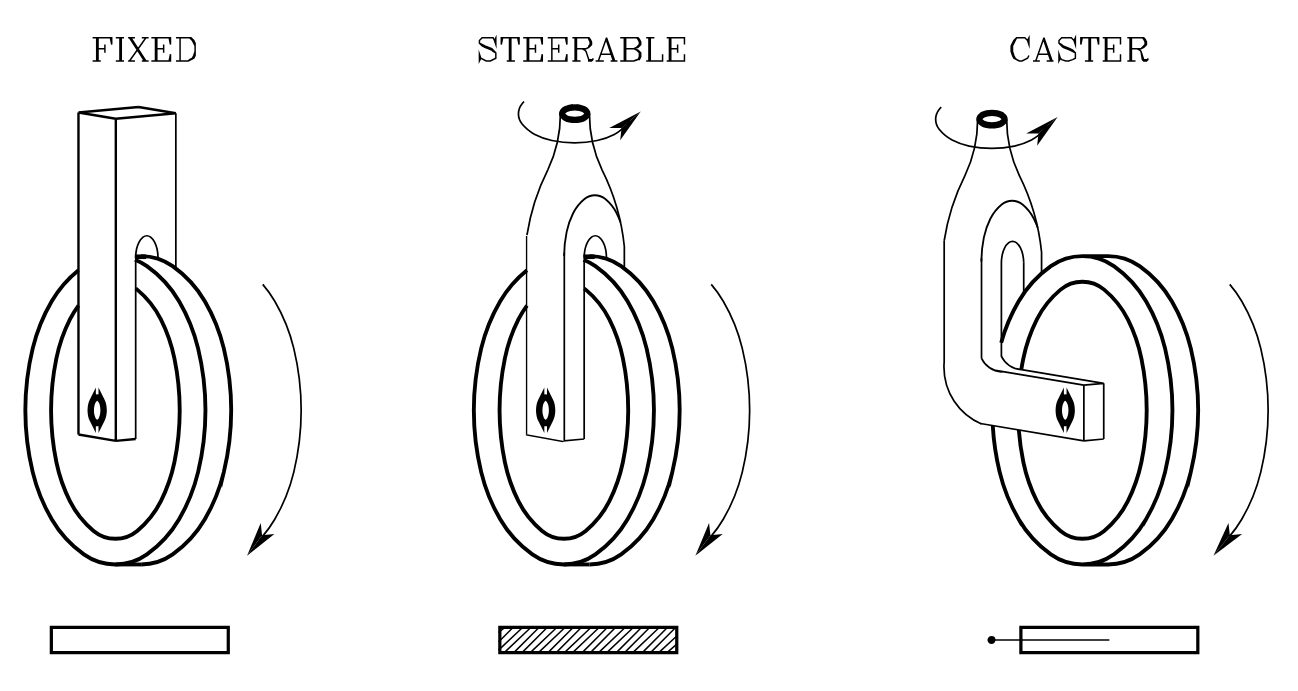
\includegraphics[width=150mm, keepaspectratio]{figures/021_wheels.png}
    \caption{Kerék mechanizmusok \cite{siciliano2010robotics}}
    \label{fig:wheels}
\end{figure}

\begin{itemize}
    \item \emph{Fix kerekek (fixed)}: csak irányban forognak (előre-hátra), nem képesek elfordulni oldalirányban. Általában meghajtott kerekek tartoznak ide, amelyek a robot hajtását biztosítják, például egy autó hátsó tengelyére szerelt kerekek. A robot bázisához mereven csatlakoznak és saját tengelyük körül forognak, amely ortogonális a kerék síkjára.\cite{siciliano2010robotics}
    \item \emph{Kormányozható (steerable) kerekek}: oldalirányban elfordíthatók, a haladási irányuk megváltoztatható, például autó első tengelyén lévő kerekek. A robot bázisához egy csuklóval csatlakoznak, mely lehetővé teszi a kerekek elfordulását, illetve erre merőleges saját tengellyel rendelkeznek (szintén merőleges a kerék síkjára), melyek körül forognak.\cite{siciliano2010robotics}
    \item \emph{Szabadonfutó (bolygó/caster) kerekek}: hasonló mechanikai csatlakozással rendelkeznek, mint az irányítható kerekek, azonban a robot bázisához való csatlakozásuknál található tengely körül szabadon fordulnak el, például irodai székek vagy bevásárló kocsi kerekei. A vertikális tengely nem metszi a kerék elfordulási tengelyét hanem egy "offset" távolságra helyezkedik el. Ezek a kerekek mechanikai stabilitásban segítik a robot bázist.\cite{siciliano2010robotics}
\end{itemize}

\subsection{Mobil kerekes robotok kinematikai modellje}
Kétféle csoportosítás különíthető el: holonomikus (nem tud mozogni a sík bármelyik irányában) és omnidirekcionális (tetszőleges irányba képes mozogni). Omnidirekcionális robotok mecanum (másik nevén svéd) kerekekkel (\refstruc{fig:023_omni_wheel}) felszerelt robotok, melyek több forgó alkatrésszel rendelkeznek, a kerék kerületen mentén független elfordulni képes görgők vannak amik segítségével oldalazó mozgást is végezhet a kerék tengelyével párhuzamosan. \cite{siciliano2010robotics} \cite{ros2_control_docs}

\begin{figure}[!ht]
    \centering
    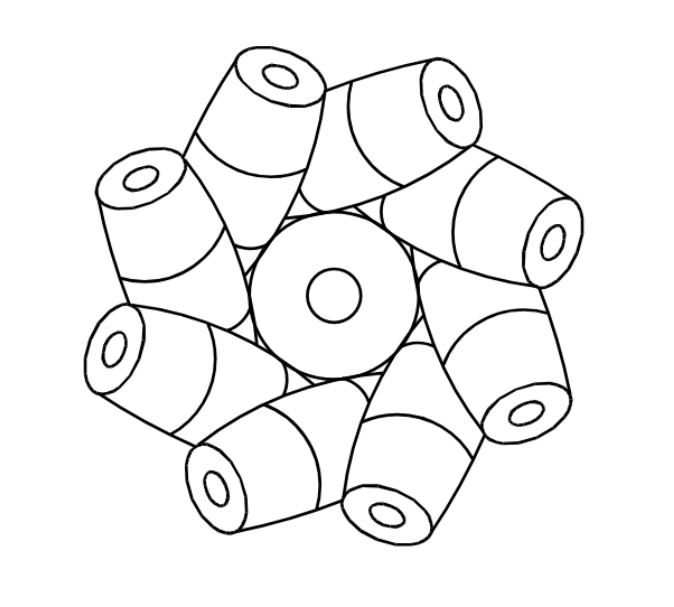
\includegraphics[width=75mm, keepaspectratio]{figures/023_omni_wheel.png}
    \caption{Mecanum kerék \cite{siciliano2010robotics}}
    \label{fig:023_omni_wheel}
\end{figure}

A dolgozatban vizsgált robotmodellek holonomikusak. Több fajta (előző pontban tárgyalt) kerék elrendezéssel hozható létre ilyen robotmodell. Klasszikusan a tricikli modell (\refstruc{fig:024_tricikli_car}), amely egy tengelyen két együttesen meghajtott kerékkel rendelkezik és egy kormányzott kerékkel. Az autókhoz hasonló modellek négy kerékkel (\refstruc{fig:024_tricikli_car}) ahol ebből kettő meghajtott és kettő kormányozható, vagy kettő egyszerre kormányozható és meghajtott plusz kettő stabilitásban asszisztáló fix kerékkel. Differenciál hajtású mobil robotok (\refstruc{fig:025_diff_model}) is a holonomikus robotok közé tartoznak, melyek két függetlenül meghajtott kerékkel és egy vagy több szabadon elforduló kerékkel szerelnek fel.  \cite{siciliano2010robotics} \cite{ros2_control_docs}

\begin{figure}[!ht]
    \centering
    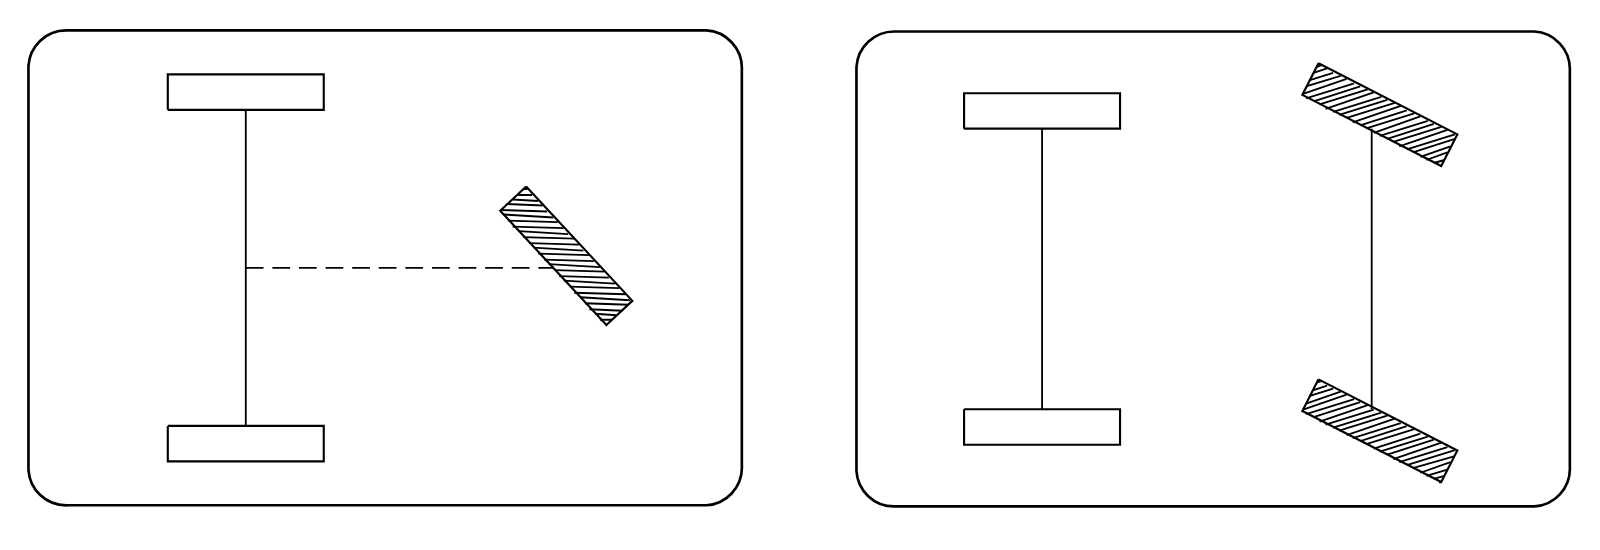
\includegraphics[width=150mm, keepaspectratio]{figures/024_tricikli_car.png}
    \caption{Tricikli és autó modellek \cite{siciliano2010robotics}}
    \label{fig:024_tricikli_car}
\end{figure}

\subsection{Differenciál hajtású robotok}
A diplomamunka során használt robotok közül mindegyik ebbe a kategóriába esik. Két szeparáltan meghajtott kerekének köszönhetően egyhelyeben képes megfordulni. A forgás tengelye a két kerék tengelyének közzéppontja. A passzív caster kerék vagy kerekek a stabilitásban segítenek, ezek lekövetik a robot mozgását. Ugye egy sík három pontból már felírható ezért a robot statikai egyensúlya nem jelent problémát, amíg a tömegközéppont vetülete a három vagy több kerek talajal való találkozási pontjainak egyenes szakaszokkal összekötő polinom belsejében marad. Mint mobil robot a differenciál hajtású szerkezetek munkatere virtuálisan végtelen, ha a munkateret a környezet egy altereként értelmezzük. A valóságban természetesen előjönnek olyan korlátok, mint a robot fizikai kiterjedése és a környezetben lévő akadályok relatív mérete és pozíciója. Természetesen itt sík felületet feltételezve (és kizárva lépcsőket, lifteket stb.) Mint nem omnidirekcionális robotmodell a lokális elmozdulására esnek korlátok. Nem tud rögtön a hajtott kerekek tengelyére merőleges irányába elmozdulni, ehhez szükséges fordulnia. De képesnek tekinthető bármely pozíciót felvenni csak nem rögtön. Ez úgy is kifejezhető, hogy a robot szabadsági fokainak száma alacsonyabb, mint a pozíciót leíró vektor változói. \cite{siciliano2010robotics} \cite{ros2_control_docs}

\begin{figure}[!ht]
    \centering
    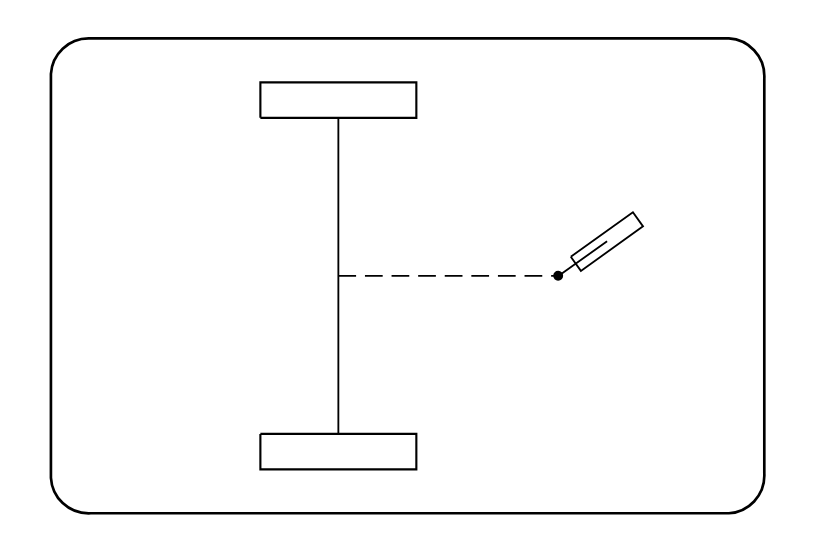
\includegraphics[width=75mm, keepaspectratio]{figures/025_diff_model.png}
    \caption{Differenciál hajtűsú robot modell \cite{siciliano2010robotics}}
    \label{fig:025_diff_model}
\end{figure}

TODO: előnyök, hátrányok más robotmechanizmusokkal szemben \\
TODO: turtlebot példa (kép)

Mozgásegyenletei felírásakor egyszerűsítve a modellt a bolygó kereket elhagyva.

\begin{figure}[!ht]
    \centering
    \includesvg[scale=1.2]{figures/022_diff_drive.svg}
    \caption{Differenciál hajtású robot 2 dimenzióban \cite{ros2_control_docs}}
    \label{fig:022_diff_drive}
\end{figure}

\begin{align}
    v_{b,x}      & = \frac{v_{right} + v_{left}}{2}, \\
    \omega_{b,z} & = \frac{v_{right} - v_{left}}{w},
\end{align}

\begin{align}
    v_{left}  & = v_{b,x} - \omega_{b,z} w / 2, \\
    v_{right} & = v_{b,x} + \omega_{b,z} w / 2,
\end{align}


% Bibliográfia [Bibliography]
\addcontentsline{toc}{chapter}{\bibname}
{
    \footnotesize  % Kisebb betűméret [Smaller font size]
    \bibliography{bib/mybib}
}


% Idegen nyelvű (angol) összefoglaló [Foreign language summary]
\include{chapters/summary-foreign}


% Függelék és mellékletek [Appendices]
%\excludeFromLocAndLot % A következő ábrákat és a táblázatokat hagyja ki a jegyzékből
% [Exclude following figures and tables from List Of Figures/Tables]

\include{chapters/appendices}        % Függelék - opcionális
\include{chapters/annexes}           % Mellékletek

\end{document}
